%!TEX root = ../template.tex
%%%%%%%%%%%%%%%%%%%%%%%%%%%%%%%%%%%%%%%%%%%%%%%%%%%%%%%%%%%%%%%%%%%%
%% my-chapter1.tex
%% NOVA thesis document file
%%
%% Chapter with the template manual
%%%%%%%%%%%%%%%%%%%%%%%%%%%%%%%%%%%%%%%%%%%%%%%%%%%%%%%%%%%%%%%%%%%%
%\usepackage{amsmath}
%\usepackage[table]{xcolor}
%\usepackage{xltabular}
%%\usepackage{colortbl} % Added this line
%\usepackage{booktabs}
%\usepackage{enumitem}
%\usepackage{tikz}
%\usetikzlibrary{shapes, arrows, positioning, fit}


\typeout{NT FILE mfc.tex}%

\chapter{Computational Financial Mathematics}
\label{ch:comp_fin_math}

    This assignment for the Computational Financial Mathematics course explores and applies various financial
    modelling and computational techniques.
    The project encompasses key topics such as financial mathematics, discrete-time and continuous-time modelling,
    partial differential equations, Monte Carlo simulation, and sensitivity analysis.
    The Binomial model for option pricing will be examined, and the Black-Scholes model will be derived and implemented.
    Option pricing problems will be solved using PDEs,
    and Monte Carlo simulations will be used to model asset price evolution.
    The Greeks for European options will be computed.
    Practical examples and computational implementations will be demonstrated using Python,
    ensuring a comprehensive understanding of the concepts covered.

\section{Financial Mathematics}
    \label{sec:fin_math}

%    Review and describe the main concepts of financial mathematics,
%    namely the concepts of Equities, Commodities, Forwards, Futures and Options.

    Financial mathematics is a branch of applied mathematics that deals with financial markets and instruments.
    It is a fundamental tool for understanding and analysing financial markets, pricing financial instruments,
    and managing financial risk.
    Key examples include equities, commodities, forwards, futures, and options.
    These concepts are essential for understanding the functioning of financial markets and the valuation of
    financial instruments.
    They are built upon core concepts such as the time value of money, risk and return, and arbitrage.
    Financial mathematics provides the tools and models to analyse these assets and understand their behaviour in the market.

    \subsection{Equities}
        \label{sec:equities}

        Equities, also known as stocks or shares, represent ownership in a company.
        When an investor buys shares of a company,
        they become a part-owner of the company and are entitled to a share of the company's profits.
        Equities are traded on stock exchanges, and their prices are determined by supply and demand in the market.
        Traditional Equity investors can make money through:

        \begin{enumerate}
            \item Capital appreciation: Investors buy shares with the expectation that the value will increase over time,
                allowing them to sell at a higher price and realise a profit.
            \item Dividends: Companies distribute a portion of their profits to shareholders in the form of dividends.
            \item Short selling: Investors can also make money by selling borrowed shares with the intention of buying
                them back at a lower price.
        \end{enumerate}

        In addition to traditional equity investments,
        investors can also invest in equity derivatives, such as options and futures,
        which allow them to speculate on the price movements of equities without owning the underlying shares.

    \subsection{Forwards}
        \label{sec:forwards}

        A forward contract is a financial agreement between two parties to buy or sell an asset at a predetermined price,
        with the transaction set to occur at a specified future date.
        The contract price is established at the time the agreement is initiated.
        Forward contracts play a significant role in managing financial risk,
        particularly as a hedge against adverse price fluctuations,
        while also serving as a vehicle for speculation on future pricing trends.
        One of the key advantages of forward contracts lies in their flexibility,
        as they can be tailored to the unique requirements and preferences of the parties involved.

    \subsection{Futures}
        \label{sec:futures}

        A futures contract shares similarities with a forward contract in its purpose and structure;
        however, it differs by being standardised and traded on a regulated exchange.
        These standardised terms ensure greater transparency and facilitate market efficiency.
        Futures contracts are widely used in financial markets for two primary purposes: hedging,
        where they help mitigate the risks associated with price fluctuations, and speculation,
        where they allow participants to express views on future price movements\cite{hull_options_2012}. \\

        One of the primary advantages of futures contracts is their high liquidity,
        stemming from the fact that they can be easily bought or sold on an exchange.
        This liquidity enhances their appeal to market participants,
        particularly those seeking flexibility in managing risk or capitalising on market opportunities.
        Moreover, these instruments are used across a broad spectrum of markets, encompassing commodities, equities,
        and interest rate derivatives, highlighting their versatility and significance in modern financial markets. \\

        Table~\ref{tab:futures_forwards} outlines the key differences between futures and forwards contracts:

        \begin{xltabular}{\textwidth}
            {   % This is the column specification for the table
                >{\ttfamily\raggedleft\arraybackslash}m{0.33\textwidth}
                >{\ttfamily\centering\arraybackslash}m{0.33\textwidth}
                >{\ttfamily\centering\arraybackslash}m{0.33\textwidth}
            }
            \hline
                                & \textbf{Futures} & \textbf{Forwards} \\
                \hline
            \textbf{Contract}    & Highly standardized & Custom \\
                \hline
            \textbf{Exchange}    & Established & OTC \\
                \hline
            \textbf{Mark to Mkt} & Yes & No \\
                \hline
            \textbf{Settled @}   & Ending price ($P_T$) & Contract price ($F_0$) \\
                \hline
            \textbf{Credit risk} & No (counter party is clearinghouse) & Yes \\
                \hline
            \textbf{Duration}    & Traded continuously & Held until maturity \\
                \hline
            \textbf{Cash flow}   & Daily + Margin Req. & At delivery \\
            \hline
            \label{tab:futures_forwards}
        \end{xltabular}

    \subsection{Commodities}
        \label{sec:commodities}

        Commodities represent fundamental raw materials or primary agricultural products
        that serve as the foundation of global trade and economic activity.
        Examples include metals such as gold, energy resources like oil,
        and agricultural products such as wheat and coffee. These assets are traded on organised commodity exchanges,
        where their prices are governed by the dynamic interplay of supply and demand.
        The inherent volatility in commodity prices is influenced by a variety of factors,
        including weather variability, geopolitical uncertainties,
        and shifts in global economic conditions\cite{wilmott_paul_2007}.
        Understanding and modelling such price behaviour,
        particularly through quantitative methods rooted in mathematics and statistics,
        is of critical importance in developing robust risk management and trading strategies

%    In practice, turbine manufactors provide a table of values for the power output at discrete wind speeds.
%    Within the range of these two critical thresholds,
%    the relationship between wind speed and the generated energy can be represented by a polynomial relationship
%    interpolating manufactor data for each turbine model.
%    See below~\ref{eq:power_curve}, example for a 2MW turbine.
%
%    \begin{equation}
%        PC(x) =
%        \begin{cases}
%            0                             & \text{if } 0 <  x < 4 \\
%            21.78 x^2 - 147.96 x + 243.42 & \text{if } 4 \leq x \leq 13 \\
%            2000                          & \text{if } 13 < x \leq 25 \\
%            0                             & \text{if } x > 25
%        \end{cases}
%    \label{eq:power_curve}
%    \end{equation}
%
%    To properly model power generation, the wind speed data, usually taken at reference height,
%    must be adjusted to the given hub operation level of the turbine.
%    The physical law that permits the conversion of wind intensity with respect to the altitude is:
%
%    \begin{equation}
%        v_h= v_{h_0}  \cdot \left(\frac{h}{h_0}\right)^\theta \text { with } \theta=\left(\ln \frac{h}{z_0}\right)^{-1}
%    \label{eq:wind_speed_height}
%    \end{equation}
%
%    Where $v_{h}$ represents the wind speed measured at the height $h$ of the wind turbine hub
%    and $v_{h_0}$ is the known value of the wind speed at the specified height data is recorded.
%    Additionally, the parameter $z0$ is intimately connected to the site's morphological aspects wherein our
%    postulated wind turbine is positioned.
%    For instance, in the absence of any physical structures like buildings or trees,
%    the value of this parameter typically falls within the range of 0.01 to 0.001.
%    For situations involving offshore installations, the parameter is fixed at 0.0001, whereas
%    an average value of $z0 = 0.005$ is employed for an onshore implementation.
%
%    As described, seven parameters are required to fully define the power curve of a wind turbine.
%
%    \enumerate{
%        \item The cut-in wind speed, $v_{cut-in}$, below which the turbine is unable to generate power.
%        \item The cut-out wind speed, $v_{cut-out}$, above which the turbine is unable to generate power.
%        \item The rated wind speed, $v_{rated}$, at which the turbine is able to generate its maximum power.
%        \item The rated power, $P_{rated}$, which is the maximum power output of the turbine.
%        \item The power curve provided by the manufactor, which will determine the production between the threshold.
%        \item The hub height, $h$, at which the wind power is generated.
%        \item The spacial factor to diferentiate turbine surroundings.
%    }

\section{Descrite-Time Modelling: Binomial Model}
    \label{sec:desc_time}

    The Black-Scholes formula caused a shock to the financial world when it
    was published in 1973~\cite{black_pricing_1973}. Only later did the
    financial community realize that the formula was a special case of a more general theory of option pricing.
    The mathematical background based on diffusion models, coupled with a strong economic principles,
    might have seemed too complex for some practitioners at the time.
    This motivated the research for a simpler framework to price options, that would preserve important
    properties of the Black-Scholes model, such as no-arbitrage and risk-neutral pricing. \\

    The foundational work of \gls{crr}~\cite{cox_option_1979} introduced the binomial option pricing model,
    providing a discrete-time method for valuing options.
    From the perspective of numerical analysis within the Black-Scholes framework,
    the validity of the binomial approach derives from Donsker's Theorem~\cite{billingsley_convergence_1999}.
    This theorem establishes the weak convergence of suitably scaled random walks to Brownian motion.
    Specifically, as the time discretization within the binomial model is refined, as $\delta t \to 0$,
    the sequence of binomial processes converges weakly to a geometric Brownian motion.

    The binomial model became widely used as a numerical pricing tool for American and exotic options,
    when analytical solutions are not available.
    The model's simplicity and intuitive appeal made it a popular choice for teaching option pricing theory,
    as the arbitrage-free pricing principle, market completeness, and risk-neutral valuation are easily demonstrated.

    \subsection{Option Princing and the Binomial Tree}
        \label{sec:bin_tree}

    An n-period binomial tree is a discrete-time stochastic model for the dynamic evolution of an
    underlying asset's price over time. Can be represented such that
    \begin{equation}
        S^{(n)}(i+1) =
            \begin{cases}
                u S^{(n)}(i), & \text{if the price increases from period } i \text{ to } i+1, \\
                d S^{(n)}(i), & \text{if the price decreases from period } i \text{ to } i+1.
            \end{cases}
        \label{eq:equation}
    \end{equation}
    where $u$ is the up factor and $d$ is the down factor. Coupled with each upward or downward movement,
    a probability $p$ can be assigned to the up movement, and $1-p$ to the down movement,
    see Fig.~\ref{fig:binomial_tree}.

    \begin{figure}
        \centering
        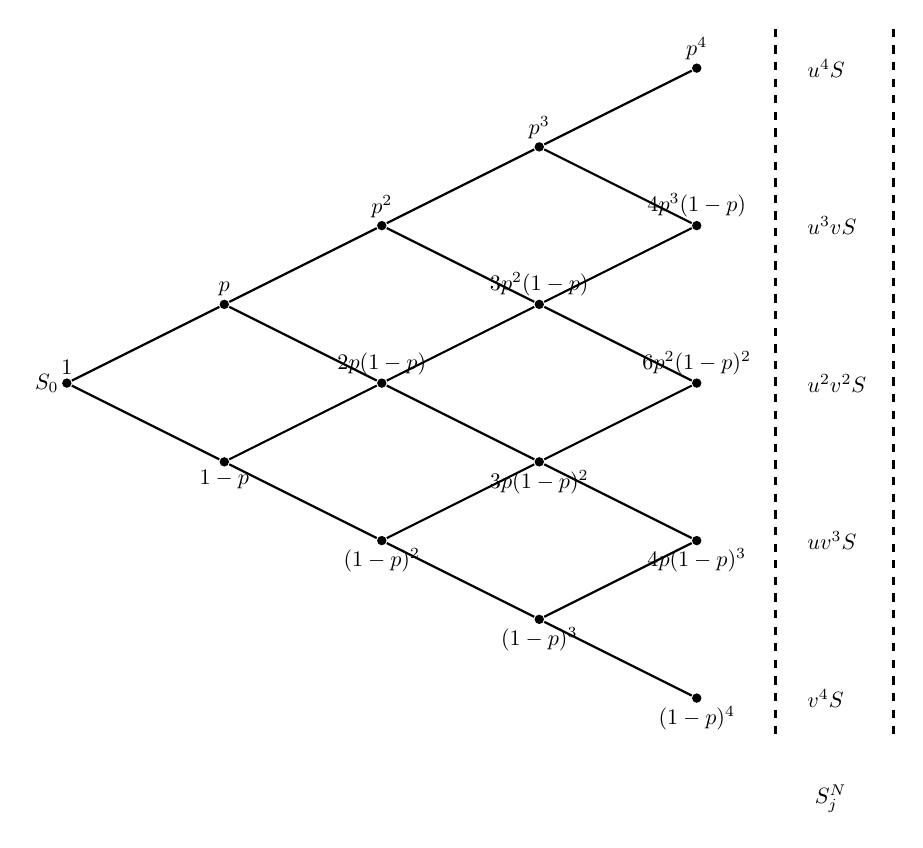
\begin{tikzpicture}[scale=1, every node/.style={scale=0.8}, every path/.style={thick}]

            % Nodes
            \node[fill=black, circle, inner sep=1.5pt] at (0,0) (N0) {};
            \node[fill=black, circle, inner sep=1.5pt] at (2,1) (N11) {};
            \node[fill=black, circle, inner sep=1.5pt] at (2,-1) (N12) {};
            \node[fill=black, circle, inner sep=1.5pt] at (4,2) (N21) {};
            \node[fill=black, circle, inner sep=1.5pt] at (4,0) (N22) {};
            \node[fill=black, circle, inner sep=1.5pt] at (4,-2) (N23) {};
            \node[fill=black, circle, inner sep=1.5pt] at (6,3) (N31) {};
            \node[fill=black, circle, inner sep=1.5pt] at (6,1) (N32) {};
            \node[fill=black, circle, inner sep=1.5pt] at (6,-1) (N33) {};
            \node[fill=black, circle, inner sep=1.5pt] at (6,-3) (N34) {};
            \node[fill=black, circle, inner sep=1.5pt] at (8,4) (N41) {};
            \node[fill=black, circle, inner sep=1.5pt] at (8,2) (N42) {};
            \node[fill=black, circle, inner sep=1.5pt] at (8,0) (N43) {};
            \node[fill=black, circle, inner sep=1.5pt] at (8,-2) (N44) {};
            \node[fill=black, circle, inner sep=1.5pt] at (8,-4) (N45) {};

            % Lines
            \draw (N0) -- (N11);
            \draw (N0) -- (N12);

            \draw (N11) -- (N21);
            \draw (N11) -- (N22);
            \draw (N12) -- (N22);
            \draw (N12) -- (N23);

            \draw (N21) -- (N31);
            \draw (N21) -- (N32);
            \draw (N22) -- (N32);
            \draw (N22) -- (N33);
            \draw (N23) -- (N33);
            \draw (N23) -- (N34);

            \draw (N31) -- (N41);
            \draw (N31) -- (N42);
            \draw (N32) -- (N42);
            \draw (N32) -- (N43);
            \draw (N33) -- (N43);
            \draw (N33) -- (N44);
            \draw (N34) -- (N44);
            \draw (N34) -- (N45);

            % Labels
            \node[above] at (N0) {$1$};
            \node[left]  at (N0) {$S_0$};
            \node[above] at (N11) {$p$};
            \node[below] at (N12) {$1-p$};

            \node[above] at (N21) {$p^2$};
            \node[above] at (N22) {$2p(1-p)$};
            \node[below] at (N23) {$(1-p)^2$};

            \node[above] at (N31) {$p^3$};
            \node[above] at (N32) {$3p^2(1-p)$};
            \node[below] at (N33) {$3p(1-p)^2$};
            \node[below] at (N34) {$(1-p)^3$};

            \node[above] at (N41) {$p^4$};
            \node[above] at (N42) {$4p^3(1-p)$};
            \node[above] at (N43) {$6p^2(1-p)^2$};
            \node[below] at (N44) {$4p(1-p)^3$};
            \node[below] at (N45) {$(1-p)^4$};


            % Payoff Values
            \node[right] at (9.3,4) {$u^4S$};
            \node[right] at (9.3,2) {$u^3vS$};
            \node[right] at (9.3,0) {$u^2v^2S$};
            \node[right] at (9.3,-2) {$uv^3S$};
            \node[right] at (9.3,-4) {$v^4S$};

            % Vertical Lines
            \draw[dashed] (9,4.5) -- (9,-4.5);
            \draw[dashed] (10.5,4.5) -- (10.5,-4.5);

            % Asset Prices Label
            \node[below] at (9.7,-5) {$S^{N}_{j}$};

        \end{tikzpicture}
        \caption{Binomial Tree for Option Pricing.}
        \label{fig:binomial_tree}
    \end{figure}

    where $S^{N}_{j}$ is the price at time step N and represents the asset price at the $j$-th tree's node.

    A relation is required $u > d$ and $S^{(n)}(0) = S_0$ is the initial price.
    A discrete-time framework is considered with equidistant time steps,
    such that $\delta t = T/n$ represents the length of each period which $T$ denotes the time to maturity
    and n is the number of periods.
    The \gls{crr} model employs a recombining binomial tree,
    achieved by imposing the condition $u = 1/d$.
    This recombination property,
    where an upward movement followed by a downward movement (or vice versa) results in the same price,
    significantly reduces the computational complexity.
    Specifically, a recombining tree with $n$ time steps contains $2n+1$ nodes,
    as opposed to $2^n$ nodes in a general non-recombining binomial tree.
    This enhanced computational efficiency makes the \gls{crr} model particularly attractive for practical applications.
    Furthermore, the recombining structure facilitates the convergence of continuous-time processes,
    such as geometric Brownian motion in the limit as $\delta t \to 0$~\cite{billingsley_convergence_1999}.

    The risk-free rate is constant and assumed to be equal to $r$.
    In addition to trading this asset,
    an investor can also invest in a back account with a continuously compounded interest rate $r$.
    Considering continuous compounding, the value of the back account grows by the factor $e^{r\delta t}$ in each period.
    The no-arbitrage principle implies that

    \begin{equation}
        u > e^{r\delta t} > d
        \label{eq:no_arbitrage_ud}
    \end{equation}

    If the above relation is violated, one can generate money without investing their own funds by either
    selling the stock short $ u < e^{r \delta t}$ or
    financing a stock purchase by a credit (in the case of $d > e^{r \delta t} $).

    The binomial method can therefore be applied as a discrete time numerical valuation of options,
    as an approximation to the Black-Scholes model.
    It is required that $p$ be chosen such that the first and second moment of the one-period log-returns is preserved,
    so that the binomial stock price framework approximates Black-Scholes.
    The parameter specification initially suggested made by \gls{crr} was

   \begin{equation}
        u = e^{\sigma \sqrt{\Delta t}}, \quad
        d = \frac{1}{u}, \quad
        p = \frac{1}{2} \left( 1 + \left( r - \frac{1}{2} \sigma^2 \right) \frac{1}{\sigma} \sqrt{\Delta t} \right)
        \label{eq:crr_parameters}
   \end{equation}

    note that the parameter $u=e^{\sigma \sqrt{\delta t}}$ comes from the need to match the variance of the
    binomial model to that of the Black-Scholes lognomal underlying price process.
    This methodology provides a closed-form expression for $u$, $d$ and $p$,
    making its implementations straightforward and computationally efficient. \\

    To implicitly include both the drift and volatility in the binomial model,
    Wilmott~\cite{wilmott_paul_2007} derives parameters $u$, $d$ and $p$ to allow more flexibility in adjusting
    for approximations or alternative assumptions.\ Despite slight differences,
    both methods follow the same principles of a lognormal underlying price process, risk-neutral valuation,
    moment matching and both require $\delta t$ to be small enough to ensure convergence to the Black-Scholes model.

    \begin{equation}
        puS + (1 - p)dS =
            SE \left[ e^{\left(\mu -\frac{1}{2} \sigma^2 \right) \delta t + \sigma \phi \sqrt{\delta t}} \right] =
            S e^{\mu \, \delta t}
        \label{eq:pw_drift}
    \end{equation}

    where $\phi$ is the standard normal random variable $\phi \sim N(0,1)$.
    Taking the expectation of S in the Black-Scholes model, we have

    \begin{equation}
        pu + (1 - p)d = e^{\mu \ \delta t}
        \label{eq:pw_s_expectation]}
    \end{equation}

    Rearranging equation~\ref{eq:pw_s_expectation]}

    \begin{equation}
        p = \frac{e^{\mu \delta t} - d}{u - d}
        \label{eq:pw_p}
    \end{equation}

    The probability $p$ here is obtained by matching the expectation of the binomial random walk with the expected
    value of the stochastic geometric Brownian motion as the underlying price process. \\

    For the binomial walk, to have the correct variance, we have again to match the variance of the binomial model
    with that of the Black-Scholes lognormal underlying price process.
    The variance is defined as $V[x] = E(x^2) - E(x)^2$.
    For both the lognormal process and the binomial walk, the variance can be expressed as follows:

    \begin{align}
        V[S] &= e^{(2\mu + \sigma^2)\delta t} - \left(e^{\mu \delta t}\right)^2 \\
        V[BinWalk] &= p u^2 + (1 - p) d^2 - \left(p u + (1 - p) d\right)^2
        \label{eq:pw_variance}
    \end{align}

    Then, from the equations~\ref{eq:pw_variance} above

    \begin{equation}
        p u^2 + (1 - p) d^2 = e^{(2\mu + \sigma^2)\delta t}
        \label{eq:pw_bw_variance}
    \end{equation}

    Using the relation to ensure node recombination $u = 1/d$, together with the equations
    ~\ref{eq:pw_p} and~\ref{eq:pw_bw_variance}, we can get the following expression for the upward factor $u$:

    \begin{equation}
        u = \frac{1}{2} \left( e^{-\mu \delta t} + e^{(\mu + \sigma^2)\delta t} \right)
            + \frac{1}{2} \sqrt{\left( e^{-\mu \delta t} + e^{(\mu + \sigma^2)\delta t} \right)^2 - 4}
        \label{eq:pw_u}
    \end{equation}

    \subsection{Binomial Option Pricing}
        \label{sec:bin_option_pricing}

    An option is a financial derivative that provides the holder with the right, but not the obligation,
    to either purchase or sell an underlying asset at a predetermined price, referred to as the strike price,
    denoted by $K$.
    The options that can only be exercised at the expiration date are known as European options,
    while those that can be exercised at any time before the expiration date are referred to as American options.
    Options are categorized into two types:
    \begin{itemize}
        \item \textbf{Call Option}: Grants the holder the right to purchase the underlying asset. \\
        The payoff is: \( \max(S_T - K, 0) \)
        \item \textbf{Put Option}: Grants the holder the right to sell the underlying asset. \\
        The payoff is: \( \max(K - S_T, 0) \)
    \end{itemize}

    The no-arbitrage principle can be extended to a generalized framework by considering a stock with an initial price
    $S_0$ and an associated option (or any derivative dependent on the stock) with a current value of $V$.
    If the stock price rises to $S_0 u$, the option's payoff is $V_u$, and if the stock price falls to $S_0 d$,
    the option's payoff is $V_d$.

    To analyze the pricing, we construct a portfolio consisting of one option and short position in a quantity $\Delta$
    of the underlying.
    The value of $\Delta$ is derived such that the portfolio becomes risk-neutral.
    A risk-free portfolio means that the value of the portfolio is the same regardless of whether
    the stock price moves up or down.
    To achieve this, we set the values of the portfolio equal in the two scenarios:

    \begin{equation}
        S_0 u \Delta- V_u = S_0 d \Delta - V_d
        \label{eq:risk_neutral}
    \end{equation}

    this means the amount of $\Delta$ should be

    \begin{equation}
        \Delta = \frac{V_u - V_d}{(u - d) S_0}
        \label{eq:delta}
    \end{equation}

    In this case, the portfolio is risk-less and, for there to be no arbitrage opportunities,
    it must earn the risk-free interest rate.
    Equation~\ref{eq:delta} shows that $\Delta$ is the ratio of the change in the option price to the change
    in the stock price as we move between the nodes at time $T$.

    By the no-arbitrage principle, the cost of setting up the portfolio must be equal to the present value of the portfolio.

    \begin{equation}
        S_0 \Delta - V = (S_0 u \Delta - V_u)e^{-rT}
        \label{eq:no_arbitrage}
    \end{equation}

    If we denote the risk-free interest rate by $r$ for the present value,
    assuming continuous discounting $e^{-rT}$.
    Rearrange the equation to get the option value $V$ and substitute $\Delta$ from equation~\ref{eq:delta}

    \begin{equation}
        V = e^{-rT} [p V_u + (1 - p) V_d]
        \label{eq:option_value}
    \end{equation}

    where

    \begin{equation}
        p = \frac{e^{rT} - d}{u - d}
        \label{eq:prob_value}
    \end{equation}

    American-style exercise can be effectively implemented within a binomial framework.
    Consider dividing the life of an American option into $N$ intervals, each of length $\Delta t$.
    The $j$th node at time $i \Delta t$ will be denoted as the $(i, j)$ node,
    where $0 \leq i \leq N$ and $0 \leq j \leq i$.
    Let $V_{i,j}$ represent the value of the option at the $(i, j)$ node.
    The underlying asset price at the $(i, j)$ node is given by $S_0 u^j d^{i-j}$.
    For a call option, its value at time $T$ (the expiration date) is expressed as

    \begin{equation}
        V_{N,j} = \max
            \left\lbrace
                S_0 u^j d^{N-j} - K, 0
            \right\rbrace, \quad j = 0, 1, \ldots, N
        \label{eq:call_option}
    \end{equation}

    As presented in~\ref{fig:binomial_tree},
    there is a probability $p$ of moving from the $(i, j)$ node at time $i \delta t$ to the $(i+1, j+1)$
    node at time $(i+1) \delta t$, and a probability $1 - p$ of moving from the $(i, j)$ node at
    time $i \delta t$ to the $(i+1, j)$ node at time $(i+1) \delta t$.
    Assuming no early exercise (European), a risk-neutral valuation gives:

    \begin{equation}
        V_{i,j} = e^{-r \Delta t} \left[ p V_{i+1, j+1} + (1 - p) V_{i+1, j} \right]
        \label{eq:european_option}
    \end{equation}

    for $0 \leq i \leq N-1$ and $0 \leq j \leq i$.
    To take account of early exercise (American),
    this value for $V_{i,j}$ must be compared with the option's intrinsic value, so that for a call:

    \begin{equation}
        V_{i,j} = \max
            \left\lbrace
                S_0 u^j d^{i-j} - K, \, e^{-r \Delta t} \left[ p V_{i+1, j+1} + (1 - p) V_{i+1, j} \right]
            \right\rbrace
        \label{eq:american_call_option}
    \end{equation}

    The primary distinction between European and American option pricing lies in the ability to exercise
    an American option at any point prior to expiration.
    Consequently, at each node in the pricing model,
    the value of the option must be compared to its intrinsic value to determine whether early exercise is optimal.

    Below is a Python code snippet that implements the binomial option pricing model for the American option.
    The European option is also implemented in the same way, using equation~\ref{eq:european_option} instead.
    To implement the model efficiently, the code uses the NumPy library and operations are fully vectorized.
    Due the recursive nature of the model, the code uses a backward induction approach to calculate the option price.

    \begin{lstlisting}[
       language=Python,
       caption={Python Code: American\_option\_price},
       label={lst:american_option_price}
    ]
def american_option_price(S0, sigma, r, K, T, N, option_type):
   # Time step
   dt = T / N

   # Discount factor
   disc = np.exp(-r * dt)

   # Up and down factors
   temp1 = np.exp((r + sigma ** 2) * dt)
   temp2 = 0.5 * (temp1 + disc)
   u = temp2 + np.sqrt(temp2 ** 2  - 1)
   d = 1 / u

   # Probability
   p = (np.exp(r * dt) - d) / (u - d)

   # Generate stock prices at maturity
   j = np.arange(N + 1)
   S = S0 * (u ** j) * (d ** (N - j))

   payoff = (S - K) if option_type == "call" else (K - S)
   v_mat = np.maximum(payoff, 0)

   V = np.zeros((N + 1, N + 1))
   V[:,-1] = v_mat

   # Backward induction through the tree
   for n in range(N - 1, -1, -1):
       # Adjust stock prices from the previous step
       S = S[:-1] / d
       start_idx = N - n
       end_idx = -N-1+n

       disc_value = (
           p * V[start_idx:, n+1] + (1 - p) * V[start_idx-1:-1, n+1]
       ) * disc

       # Calculate payoff based on option type
       payoff = (S - K) if option_type == "call" else (K - S)

       # Update option values
       V[start_idx:, end_idx] = np.maximum(disc_value, np.maximum(payoff, 0))

   # Return the option values in a upper triangular matrix
   return V[::-1]
   \end{lstlisting}


    

\section{Continuous-Time Modelling}
    \label{sec:cont_time}

    The focus of this section is to model wind power generation based on historical real and forecasted data.
    Conventional assumptions, like data independence and identically distribution, fall short when handling time-stamped
    data streams influenced by multifaceted predictors or features.
    This challenge necessitates the application of time series models to capture the inherent temporal dependencies,
    such as those stemming from macroeconomic indicators, enterprise operation, market dynamics, and weather conditions.\\

    One interest of this thesis is to explore recent techniques that work well for feature selection problems in
    time series applications.
    A technique that can join Bayesian inference with time series models is the~\gls{bsts}.
    Initially introduced and further explored by Scott and Varian~\cite{scott_predicting_2013, scott_bayesian_2013},
    the~\gls{bsts} model is a powerful tool for feature selection,
time series forecasting, and inferring causal relationships. \\


\section{Partial Differential Equations}
    \label{sec:pde}

    The focus of this section is to model wind power generation based on historical real and forecasted data.
    Conventional assumptions, like data independence and identical distribution, fall short when handling time-stamped
    data streams influenced by multifaceted predictors or features.
    This challenge necessitates the application of time series models to capture the inherent temporal dependencies,
    such as those stemming from macroeconomic indicators, enterprise operation, market dynamics, and weather conditions.\\

    One interest of this thesis is to explore recent techniques that work well for feature selection problems in
    time series applications.
    A technique that can join Bayesian inference with time series models is the~\gls{bsts}.
    Initially introduced and further explored by Scott and Varian~\cite{scott_predicting_2013, scott_bayesian_2013},
    the~\gls{bsts} model is a powerful tool for feature selection,
time series forecasting, and inferring causal relationships. \\


\section{Monte Carlo Simulation}
    \label{sec:mc_sim}

    The focus of this section is to model wind power generation based on historical real and forecasted data.
    Conventional assumptions, like data independence and identically distribution, fall short when handling time-stamped
    data streams influenced by multifaceted predictors or features.
    This challenge necessitates the application of time series models to capture the inherent temporal dependencies,
    such as those stemming from macroeconomic indicators, enterprise operation, market dynamics, and weather conditions.\\

    One interest of this thesis is to explore recent techniques that work well for feature selection problems in
    time series applications.
    A technique that can join Bayesian inference with time series models is the~\gls{bsts}.
    Initially introduced and further explored by Scott and Varian~\cite{scott_predicting_2013, scott_bayesian_2013},
    the~\gls{bsts} model is a powerful tool for feature selection,
time series forecasting, and inferring causal relationships. \\


\section{Sensitity Analysis}
    \label{sec:sens_analysis}

    The focus of this section is to model wind power generation based on historical real and forecasted data.
    Conventional assumptions, like data independence and identically distribution, fall short when handling time-stamped
    data streams influenced by multifaceted predictors or features.
    This challenge necessitates the application of time series models to capture the inherent temporal dependencies,
    such as those stemming from macroeconomic indicators, enterprise operation, market dynamics, and weather conditions.\\

    One interest of this thesis is to explore recent techniques that work well for feature selection problems in
    time series applications.
    A technique that can join Bayesian inference with time series models is the~\gls{bsts}.
    Initially introduced and further explored by Scott and Varian~\cite{scott_predicting_2013, scott_bayesian_2013},
    the~\gls{bsts} model is a powerful tool for feature selection,
time series forecasting, and inferring causal relationships. \\



%    Structural time series models are a class of state space models that decompose a time series into several components of interest.
%    They have a considerable intuitive appeal, particularly for economic and social times.
%    Furthermore, they provide a clear link with regressions' models, both in their technical formulation and in the model selection
%    methodology that they employ~\cite{harvey_forecasting_1990}. \\
%
%    The key to handling structural time series models is the state space representation, with the state of the system
%    representing the unobserved components of the time series, such as trends and seasonal effects.
%    Once in the state space, the Kalman filter plays a fundamental role as it recursively computes the predictive distribution
%    of the state variables, given the observations up to that point in time.
%
%    Initially introduced by Jammalamadaka et al.~\cite{qiu_multivariate_2018}, the~\gls{bsts} can be extended to a multivariate
%    time series model, which is particularly useful for the analysis of multiple time series that are related to each other.
%    The~\gls{mbsts} can be used to explicitly model the correlations between different asset returns in a portfolio through
%    the covariance structure specified by $\Sigma_{t}$, see equation~\ref{eq:mbsts_obs}.
%
%\subsection{The \gls{mbsts} model}
%    \label{sec:mbsts}
%
%    Models of structural time series, exemplified by the~\gls{mbsts},
%    are categorized under state space models tailored for time series data. They are represented by the ensuing equations:
%
%    \begin{align}
%        y_{t} &= Z_{t} \alpha_{t} + \varepsilon_{t}, \qquad \varepsilon_{t} \sim N_{m}(0, \Sigma_{t})
%        \label{eq:mbsts_obs}\\
%        \notag \\
%        \alpha_{t+1} &= T_{t} \alpha_{t} + R_{t} \eta_{t}, \qquad \eta_{t} \sim N_{q}(0, Q_{t})
%        \label{eq:mbsts_trans}
%    \end{align}
%
%
%    Equation~\ref{eq:mbsts_obs} is the observation equation, which relates the $m \times 1$
%    vector of observations at time $t$ $y_{t}$ to the $d \times 1$ unobserved latent states $\alpha_{t}$,
%    where $d$ is the total number of latent states.
%    The $m \times p$ matrix of coefficients $Z_{t}$ links the unobserved factors and regressions' effects
%    with the observations' vector $y_{t}$.
%    The $m \times 1$ is the vector of observation disturbances $\varepsilon_{t}$ and are assumed to have zero means and
%    represented by a variance-covariance matrix $\Sigma_{t}$ of the order $m \times m$.\\
%
%    The second equation~\ref{eq:mbsts_trans} is the transition equation, which describes the evolution of the state vector
%    $\alpha_{t}$ over time, characterized by the $d \times d$ transition matrix $T_{t}$.
%    The $d \times q$ matrix of coefficients $R_{t}$ is often referred to as the control matrix.
%    The matrix $\eta_{t}$ is an $q \times 1$ error vector,
%    with a state diffusion matrix $Q_{t}$ of the order $q \times q$, where $q \leq d$.
%    In many standard cases, $q = d$ and $Q_{t}$ is the identity matrix $I_{d}$.
%    Although matrix $Q_{t}$ can be specified freely,
%    it is often composed of a selection from the $q$ columns of the identity matrix $I_{d}$~\cite{commandeur_introduction_2007}.\\
%
%    In summary, the~\gls{mbsts} model is defined by the following set of parameters:
%
%    \begin{itemize}
%        \item $y_{t}$ ($m \times 1$): Observations at time $t$
%        \item $\alpha_{t}$ ($d \times 1$): Unobserved latent states $d$
%        \item $Z_{t}$ ($m \times p$): Coefficients linking the unobserved factors and regression effects
%            with the observations vector $y_{t}$
%        \item $\varepsilon_{t}$ ($m \times 1$): Observation disturbances, assumed to have zero means,
%            represented by the variance-covariance matrix $\Sigma_{t}$
%        \item $T_{t}$ ($d \times d$): Transition matrix characterizing the evolution of the state vector $\alpha_{t}$
%        \item $R_{t}$ ($d \times q$): Control matrix of coefficients
%        \item $\eta_{t}$ ($q \times 1$): Error vector with a state diffusion matrix $Q_{t}$ of the order $q \times q$ where $q \leq d$
%        \item $\Sigma_{t}$ ($m \times m$): Covariance matrix of the order $m \times m$ representing the observation disturbances
%        \item $Q_{t}$ ($q \times q$): State diffusion matrix
%    \end{itemize}
%
%    As per developed by Harvey~\cite{harvey_forecasting_1990}, a basic structural time series model can be represented
%    by a direct interpretation of its underlying components.
%    In a general, the model can be expressed as:
%
%    \begin{equation}
%        y_{t} = \mu_{t} + \theta{t} + \omega_{t} + \xi_{t} + \varepsilon_{t} ,
%        \qquad \varepsilon_{t} \sim N_{m}(0, \Sigma_{\varepsilon}), \quad t = 1, 2, ..., n
%    \label{eq:sts}
%    \end{equation}
%
%    where $y_{t}$, $\mu_{t}$, $\theta{t}$, $\omega_{t}$, $\xi_{t}$ and $\varepsilon_{t}$ are m-dimension vectors,
%    representing targeted time series, linear trend, seasonal, cyclical and regression components
%    with the observation disturbances respectively.
%    For simplicity, $\Sigma_{\varepsilon}$ is a $m \times m$, positive definite matrix and assumed to be constant over time.
%
%    Elucidating further on the state space form, $\alpha_{t}$ aggregates these multifaceted components,
%    depicting the concealed and unobserved latent states, such that:
%
%   \begin{equation}
%        \alpha_{t} = [\mu_{t}, \theta_{t}, \omega_{t}, \xi_{t}]^T
%    \label{eq:sts_latent}
%    \end{equation}
%
%
%    In the prevailing model, each component of the state is compiled individually,
%    where every component produces an incremental influence on $y_{t}$.
%    The adaptability of this model facilitates the incorporation of various model elements specific to each target series.
%
%    % Develope the different components states
%\subsection{State Components}
%    \label{sec:state_components}
%
%    A structural time series model is composed of several components, each representing a distinct aspect of the time series,
%    allowing to add flexibility and contributing to the overall model's predictive capabilities.
%    The model components are typically divided into four main categories: trend, seasonal, cyclical and regression components.
%    In the current model formulation, components are modelled explicitly and are assembled independently,
%    with each yielding an additive contribution to $y_{t}$.
%
%\subsubsection{Trend Component}
%    \label{sec:trend_component}
%
%    The trend component is a fundamental element of the structural time series model.
%    It represents the long-term movement of the time series, capturing the underlying growth or decline over time.
%    The trend component is typically modelled as a linear or non-linear function of time.
%    The linear trend component can be portrait as:
%
%%    \begin{gather}
%%        \bm{\mu}_{t+1} = \bm{\mu}_{t} + \bm{\delta}_{t} + \bm{u}_{t},
%%            \qquad \bm{u}_{t} \stackrel{\textit{iid}}{\sim} N_{m}(0, \bm{\Sigma}_{\mu}) \\
%%        \notag \\
%%        \bm{\delta}_{t+1} = \bm{d} + \bm{P}(\bm{\delta}_{t} - \bm{d}) + \bm{v}_{t},
%%            \qquad \bm{v}_{t} \stackrel{\textit{iid}}{\sim} N_{m}(0, \bm{\Sigma}_{\delta})
%%        \label{eq:group}
%%    \end{gather}
%
%    \begin{equation}
%        \bm{\eta}_{t+1}=
%            \bm{T}_{T} \bm{\eta}_{t} + \bm{G}_{T} \bm{\gamma} + \bm{\omega}_{T,t}
%        \label{eq:trend_state}
%    \end{equation}
%
%    where:
%    \begin{itemize}
%        \item $\bm{T}_T$ $(2m \times 2m)$ transition matrix that applies the learning rate $\rho$
%        \item $\bm{\eta}_{t}$ $(2m \times 1)$ state vector that contains the trend components for all time series at time $t$
%        \item $\bm{G}_T$ $(2m \times 1)$ transition vector that applies the long-term slope $\gamma$
%        \item $\bm{\gamma}$ $(m \times 1)$ is the long-term slope
%        \item $\bm{\omega}_{T,t}$ $(2m \times 2m)$ is the trend disturbance at time $t$,
%            where $w_{T,t} \sim \mathcal{N}(0, \bm{\Sigma}_{T})$
%    \end{itemize}
%
%    The updated state equation becomes, for times series $i$, can be represented as:
%
%    \begin{equation}
%        \left[
%            \begin{array}{c}
%                \mu_{t+1}^{(i)} \\
%                \delta_{t+1}^{(i)}
%            \end{array}
%        \right] =
%        \left[
%            \begin{array}{cc}
%                1 & 1 \\
%                0 & \rho^{(i)}
%            \end{array}
%        \right]
%        \left[
%            \begin{array}{c}
%                \mu_{t}^{(i)} \\
%                \delta_{t}^{(i)}
%            \end{array}
%        \right] +
%        \left[
%            \begin{array}{c}
%                0 \\
%                1 - \rho^{(i)}
%            \end{array}
%        \right]
%        \gamma^{(i)} +
%        \left[
%            \begin{array}{c}
%                \omega_{t}^{(\mu,i)} \\
%                \omega_{t}^{(\delta,i)}
%            \end{array}
%        \right]
%        \label{eq:state_update}
%    \end{equation}
%
%    The combined transition matrix $\bm{T}_T$ for $m$ time series is a block-diagonal matrix:
%
%    \begin{equation}
%        \mathbf{T}_T=
%            \left[
%                \begin{array}{cccc}
%                    \mathbf{T}_{T, 1} & \mathbf{0}        & \cdots & \mathbf{0} \\
%                    \mathbf{0}        & \mathbf{T}_{T, 2} & \cdots & \mathbf{0} \\
%                    \vdots            & \vdots            & \ddots & \vdots     \\
%                    \mathbf{0}        & \mathbf{0}        & \cdots & \mathbf{T}_{T, m}
%                \end{array}
%            \right]
%        \label{eq:state_transition_mv}
%    \end{equation}
%
%    where each block of the diagonal matrix is a $(2 \times 2)$ for one time series,
%    represented in equation~\ref{eq:state_update}.
%    The model features a parameter $\bm{\rho}$ $(0 < \bm{\rho}^{(i)} < 1)$ which represents the learning rate
%    that underlies the local trend update process, providing the ability to balance short-term and long-term information.
%    Specifically, when $\bm{\rho}^{(i)} = 1$, the model induces a random walk within the associated slope,
%    leading to a non-stationary trend component.
%
%    The state vector $\bm{\eta}_{t}$ contains the trend components for all time series at time $t$.
%    When considering $m$ time series, the overall state vector is a concatenation of the state vectors for each
%    individual time series.
%
%    \begin{equation}
%        \bm{\eta}_{t}^{(i)}=
%            \left[
%                \begin{array}{c}
%                    \mu_{t}^{(1)} \\
%                    \delta_{t}^{(1)} \\
%                    \mu_{t}^{(2)} \\
%                    \delta_{t}^{(2)} \\
%                    \vdots \\
%                    \mu_{t}^{(m)} \\
%                    \delta_{t}^{(m)}
%                \end{array}
%            \right]
%        \label{eq:trend_state_vector}
%    \end{equation}
%
%    The aggregate disturbance term $\bm{\omega}_{T,t}$ is assumed to be a white noise variable with a multivariate normal distribution
%    with a covariance matrix $\bm{\Sigma}_{T}$ of the order $(2m \times 2m)$.\ The covariance matrix $\bm{\Sigma}_{T}$
%    is a block-diagonal matrix, where each block of the diagonal matrix are assumed to be independent.
%    The combined covariance matrix $\bm{\Sigma}_{T}$ can be represented as:
%
%    \begin{equation}
%        \bm{\Sigma}_{T} =
%            \left[
%                \begin{array}{cc}
%                    \mathbf{\Sigma}_{\mu} & \mathbf{0} \\
%                    \mathbf{0}            & \mathbf{\Sigma}_{\delta}
%                \end{array}
%            \right]
%        \label{eq:trend_covariance}
%    \end{equation}
%
%    Where:
%    \begin{itemize}
%        \item $\mathbf{\Sigma}_{\mu}$ covariance matrix of the trend disturbances $\omega_{t}^{(\mu,i)} \sim \mathcal{N}_{m}(0, \bm{\Sigma}_{\mu})$
%        \item $\mathbf{\Sigma}_{\delta}$ covariance matrix of the trend increments $\omega_{t}^{(\delta,i)} \sim \mathcal{N}_{m}(0, \bm{\Sigma}_{\delta})$
%    \end{itemize}
%
%\subsubsection{Seasonality}
%    \label{sec:seasonality_component}
%
%    Whenever a time series consists of hourly, quarterly or yearly data, it is common to observe a seasonal pattern.
%    The seasonal component $\bm{\tau}_{t}$ at time $t$ can be modelled using various methods,
%    such as a trigonometric form using Fourier series, categorical proxies known as "dummy variables"
%    or methods involving seasonal splines~\cite{proietti_seasonality_2023}.
%    In prevalent usage exists a model that leverages deterministic means coupled with an error term,
%    thus permitting the accommodation of alterations across time.
%    This characteristic renders this model proficient in apprehending both,
%    patterns that appear with regularity and fluctuations that are more sporadic,
%    thereby establishing robustness when applied to disparate types of sequences of time that exhibit seasonality.
%
%    A seasonal effects modelled using a deterministic approach along with a white noise error term~\cite{qiu_multivariate_2018} is:
%
%    \begin{equation}
%        \bm{\tau}_{t+1} = - \sum_{k=0}^{S_{i}-2} \bm{\tau}_{t-k}^{(i)} + \bm{w}_{t}^{(i)},
%            \qquad \bm{w}_{t} = [w_{t}^{(1)}, \ldots, w_{t}^{(m)}]^{T}
%            \stackrel{\textit{iid}}{\sim} \mathcal{N}_{m}(0, \bm{\Sigma}_{\tau})
%        \label{eq:seasonal}
%    \end{equation}
%
%    where:
%    \begin{itemize}
%        \item $S_{i}$ represents the seasonal period, e.g. weekly (s=7), monthly (s=12), hourly (s=24)
%        \item $\bm{\tau}_{t}^{i}$ ($m \times (s-1)$): seasonal effect for $i$-th time series and at time $t$
%        \item $\bm{w}_{t}^{i}$ ($(m \times (s-1)) \times 1$): white noise seasonal disturbance,
%            which is assumed to follow a multivariate normal distribution: $w_{t} \sim \mathcal{N}(\bm{\Sigma}_{\tau})$
%    \end{itemize}
%
%    The transition matrix, in the univariate case, for the seasonal effects in the state space is a $(s-1) \times (s-1)$ matrix,
%    due to the sum-zero constraint over one seasonal cycle.\ The structure of the matrix is:
%
%    \begin{equation}
%        \mathbf{T}_s^{(i)}=
%            \left[
%                \begin{array}{ccccc}
%                    -1             & -1         & \cdots &  -1        & -1 \\
%                    1              & \mathbf{0} & \cdots & \mathbf{0} & \mathbf{0} \\
%                    \mathbf{0}     & 1          & \cdots & \mathbf{0} & \mathbf{0} \\
%                    \vdots         & \vdots     & \ddots & \vdots     & \vdots \\
%                    \mathbf{0}     & \mathbf{0} & \cdots & 1          & \mathbf{0}
%                \end{array}
%            \right]
%    \label{eq:seasonal_transition_uni}
%    \end{equation}
%
%    In a multivariate scenario, when there are $m$ time series each with its own seasonal components,
%    the overall transition matrix $\mathbf{T}_s$ is a block-diagonal matrix, where each block of the diagonal matrix
%    is $(s-1) \times (s-1)$ for one time matrix.
%    The combined transition matrix $\mathbf{T}_{s}$ can be represented as:
%
%    \begin{equation}
%        \mathbf{T}_s=
%            \left[
%                \begin{array}{cccc}
%                    \mathbf{T}_{s, 1} & \mathbf{0}        & \cdots & \mathbf{0} \\
%                    \mathbf{0}        & \mathbf{T}_{s, 2} & \cdots & \mathbf{0} \\
%                    \vdots            & \vdots            & \ddots & \vdots     \\
%                    \mathbf{0}        & \mathbf{0}        & \cdots & \mathbf{T}_{s, m}
%                \end{array}
%            \right]
%        \label{eq:seasonal_transition_mv}
%    \end{equation}
%
%    where $\mathbf{T}_{s}$ has the size $(m \times (s-1)) \times (m \times (s-1))$ matrix.
%    Off-diagonal elements are zero matriz with the size of $(s-1) \times (s-1)$ as it is assumed that the seasonal transition
%    for different time series is independent in this model.
%    The state vector $\bm{\tau}_t$ contains the seasonal effects for all time series at time $t$.
%    When considering $m$ time series, the overall state vector is a concatenation of the state vectors for each
%    individual time series.\ The state vector $\bm{\tau}_t$ representation is:
%
%    \begin{equation}
%        \tau_{t+1}=
%            \left[
%                \begin{array}{c}
%                    \tau_{t+1}^{(1)} \\
%                    \tau_{t+1}^{(2)} \\
%                    \hfill \vdots \hfill \\
%                    \tau_{t+1}^{(m)}
%                \end{array}\right]
%            =\left[
%                \begin{array}{l}
%                    \tau_t^{(1)}, \tau_{t-1}^{(1)}, \ldots, \tau_{t-10}^{(1)} \\
%                    \tau_t^{(2)}, \tau_{t-1}^{(2)}, \ldots, \tau_{t-10}^{(2)} \\
%                    \hfill \vdots \hfill \\
%                    \tau_t^{(m)}, \tau_{t-1}^{(m)}, \ldots, \tau_{t-10}^{(m)}
%                \end{array}
%            \right]
%        \label{eq:seasonal_state}
%    \end{equation}
%
%    The white noise error term $\bm{w}_{t}$ plays a crucial role in the seasonal component model,
%    by allowing random variations around the deterministic seasonal pattern.
%    For $m$ time series, the combined white noise term $\bm{w}_{t}$ is:
%
%    \begin{equation}
%        w_t=
%            \left[
%                \begin{array}{c}
%                    w_{t}^{(1)} \\
%                    w_{t}^{(2)} \\
%                    \vdots \\
%                    w_{t)}^{(m)}
%                \end{array}
%            \right]
%           =
%            \left[
%                \begin{array}{c}
%                    w_{t, 1}^{(1)} \\
%                    w_{t, 2}^{(1)} \\
%                    \vdots \\
%                    w_{t, (s-1)}^{(1)} \\
%                    w_{t, 1}^{(2)} \\
%                    w_{t, 2}^{(2)} \\
%                    \vdots \\
%                    w_{t, (s-1}^{(2)} \\
%                    \vdots \\
%                    w_{t, 1}^{(m)} \\
%                    w_{t, 2}^{(m)} \\
%                    \vdots \\
%                    w_{t, (s-1)}^{(m)}
%                \end{array}
%            \right]
%    \label{eq:seasonal_error}
%    \end{equation}
%
%    When considering a multivariate time series model, the white noise error term $\bm{w}_{t}$ is assumed to follow
%    a multivariate normal distribution with a covariance matrix $\bm{\Sigma}_{\tau}$ of the order $(s-1) \times (s-1)$.
%    The covariance matrix $\bm{\Sigma}_{\tau}$ is a block-diagonal matrix, where each block of the diagonal matrix are
%    assumed to be uncorrelated between different time series.
%
%    The combined covariance matrix $\bm{\Sigma}_{\tau}$ can be represented as:
%
%    \begin{equation}
%        \bm{\Sigma}_{\tau} =
%            \left[
%                \begin{array}{cccc}
%                    \mathbf{\Sigma}_{\tau, 1} & \mathbf{0}                 & \cdots & \mathbf{0} \\
%                    \mathbf{0}                & \mathbf{\Sigma}_{\tau, 2}  & \cdots & \mathbf{0} \\
%                    \vdots                    & \vdots                     & \ddots & \vdots     \\
%                    \mathbf{0}                & \mathbf{0}                 & \cdots & \mathbf{\Sigma}_{\tau, m}
%                \end{array}
%            \right]
%    \label{eq:seasonal_covariance}
%    \end{equation}
%
%\subsubsection{Cyclical}
%    \label{sec:cyclical_component}
%
%    The cyclic part of the structural time series model signifies the medium-to-long term oscillations.
%    In the context of financial mathematics, the term `financial market cycles` generally indicates repeated fluctuations
%    that don't follow a strict periodic pattern around the data series' path.
%    A model incorporating a cyclic element can effectively emulate critical characteristics often recognized in statistical analyses.
%    These include evidence of major autocorrelation, the recurrence and alternation of phases within the data,
%    the damping or amplification of cycles and the absence of long-term persistence in the data series~\cite{qiu_multivariate_2018}.
%
%    Cyclical factors are often modelled using a deterministic approach, such as a trigonometric function or a polynomial.
%    In this case, a trigonometric function is used to model the cyclical component with dumping is postulated as:
%
%    \begin{equation}
%        \bm{\omega}_{t+1} = \bm{\rho}^{(i)} \bm{T}_c^{(i)} \bm{\omega}_{t}^{(i)} + \bm{\kappa}_{t},
%            \qquad \bm{\kappa}_{t} \stackrel{\textit{iid}}{\sim} N_{m}(0, \bm{\Sigma}_{\omega})
%        \label{eq:cyclical_state}
%    \end{equation}
%
%    where:
%    \begin{itemize}
%        \item $\bm{\omega}_{t}$ ($2m \times 1$): cyclical component at time $t$
%        \item $\bm{\rho}^{(i)}$ ($m \times 1$): damping factors vector per series $i$
%        \item $\bm{T}_c^{(i)}$ ($2m \times 2m$): transition matrix for the cyclical component
%        \item $\bm{\kappa}_{t}$ ($2m \times 1$): cyclical disturbance at time $t$
%        \item $\bm{\Sigma}_{\omega}$ ($2m \times 2m$): variance of the cyclical disturbance
%    \end{itemize}
%
%    For each time series $i$, the cyclical component state vector $\bm{\omega}_{t}$ can be represented as:
%
%    \begin{equation}
%        \bm{\omega}_{t}^{(i)}=
%            \left[
%                \begin{array}{c}
%                    \alpha_{t}^{(1)} \\
%                    \beta_{t}^{(1)} \\
%                    \alpha_{t}^{(2)} \\
%                    \beta_{t}^{(2)} \\
%                    \vdots \\
%                    \alpha_{t}^{(m)} \\
%                    \beta_{t}^{(m)}
%                \end{array}
%            \right]
%        \label{eq:cyclical_state_vector}
%    \end{equation}
%
%    where the transition matrix $\bm{T_c^{(i)}}$ for the time series $i$ is:
%
%    \begin{equation}
%        \bm{T}_c^{(i)}=
%            \left[
%                \begin{array}{cc}
%                    \cos \left(\lambda_i\right) & \sin \left(\lambda_i\right) \\
%                    -\sin \left(\lambda_i\right) & \cos \left(\lambda_i\right)
%                \end{array}
%            \right]
%        \label{eq:cyclical_transition_matrix}
%    \end{equation}
%
%    The combined transition matrix for an $m$ time series model is a block-diagonal matrix,
%    where each block of the diagonal matrix is affected by its respective dampening factor $\bm{\rho}^{(i)}$ is:
%
%    \begin{equation}
%        \bm{\rho}^{(i)} \bm{T}_c^{(i)} =
%        \left[
%            \begin{array}{ccccc}
%                \rho_1 \bm{T}_c^{(1)} & \mathbf{0} & \cdots & \mathbf{0} \\
%                \mathbf{0} & \rho_2 \bm{T}_c^{(2)} & \cdots & \mathbf{0} & \\
%                \vdots & \vdots & \ddots & \vdots & \\
%                \mathbf{0} & \mathbf{0} & \cdots & \rho_m \bm{T}_c^{(m)}
%            \end{array}
%        \right]
%        \label{eq:cyclical_transition_mv}
%    \end{equation}
%
%    For the factor $\bm{\rho}^{(i)}$ be in fact dampening, should be $ 0 < \rho < 1$.
%    The frequency $\lambda_i = 2\pi/q_i $, where $q_i$ is the period such that $0 < \lambda_i < \pi$.
%    When $\lambda_i$ is 0 or $\pi$, the model degenerates to the AR(1) process.
%    The dampening factor should be strictly less than one for stationary purpose.
%    If this damping factor surpasses unity, it induces an unrestricted cyclical motion,
%    which consequently leads to an increased magnitude of the cycle in the model.~\cite{qiu_multivariate_2018}.
%    A fundamental distinction that arises between the cyclical and seasonal constituents pertains exactly to this dampening factor.
%    In the context of the cyclical component, there is a characteristic decay in its amplitude as time progresses.
%    This phenomenon can be pragmatically utilized in the analysis of time series data,
%    particularly those impacted by exogenous shocks,
%    lending valuable insights to scholars operating outside the confines of a traditional mathematical or statistical framework.
%
%
%    The combined white noise vector for the cyclical component $\kappa^{(c)}$ for $m$ time series is a vector of dimension $2m \times 1$.
%    Each element $\bm{\kappa}_{t}^{(i)}$ in this vector corresponds to the white noise term for the state variables of the cyclical component of each time series.
%
%    \begin{equation}
%        \bm{\kappa}_{t}^{(i)}=
%            \left[
%                \begin{array}{c}
%                    \kappa_{t}^{(c,1)} \\
%                    \kappa_{t}^{(c,2)} \\
%                    \vdots \\
%                    \kappa_{t}^{(c,m)}
%                \end{array}
%            \right]
%        \label{eq:cyclical_error_mv}
%    \end{equation}
%
%    Each $\bm{\kappa}_{t}^{(i)}$ is a $2 \times 1$ vector:
%
%    \begin{equation}
%        \bm{\kappa}_{t}^{(i)}=
%            \left[
%                \begin{array}{c}
%                    \kappa_{t}^{(\alpha,i)} \\
%                    \kappa_{t}^{(\beta,i)}
%                \end{array}
%            \right]
%        \label{eq:cyclical_error}
%    \end{equation}
%
%    where $\kappa_{t}^{(\alpha,i)}$ and $\kappa_{t}^{(\beta,i)}$ are the white noise terms for the state variables
%    $\alpha^{(i)}$ and $\beta^{(i)}$ respectively.
%
%    The variance-covariance matrix $\bm{\Sigma}_{\omega}$ for the white noise term $\omega_t^{(c)}$ is a block diagonal
%    matrix of dimension $2m \times 2m$.\ Each block on the diagonal corresponds to the variance-covariance matrix of the
%    white noise term for the cyclical component of each time series.
%
%    \begin{equation}
%        \bm{\Sigma}_{\omega} =
%            \left[
%                \begin{array}{cccc}
%                    \bm{\Sigma}_{\omega, 1} & \mathbf{0} & \cdots & \mathbf{0} \\
%                    \mathbf{0} & \mathbf{\Sigma}_{\omega, 2} & \cdots & \mathbf{0} \\
%                    \vdots & \vdots & \ddots & \vdots \\
%                    \mathbf{0} & \mathbf{0} & \cdots & \mathbf{\Sigma}_{\omega, m}
%                \end{array}
%            \right]
%        \label{eq:cyclical_covariance}
%    \end{equation}
%
%    Each block on the diagonal of the matrix $\bm{\Sigma}_{\omega}$ is a $2 \times 2$ matrix representing the variance-covariance
%    white noise term $\omega_t^{(\alpha, i)}$ and $\omega_t^{(\beta, i)}$:
%
%    \begin{equation}
%        \bm{\Sigma}_{\omega, i} =
%            \left[
%                \begin{array}{cc}
%                    \sigma_{\alpha, i}^2    & \sigma_{\alpha\beta, i} \\
%                    \sigma_{\alpha\beta, i} & \sigma_{\beta, i}^2
%                \end{array}
%            \right]
%        \label{eq:cyclical_covariance_block}
%    \end{equation}
%
%    By structuring the white noise terms and their variance-covariance matrix this way,
%    clearly separate the noise affecting each time series while allowing for the noise terms of the cyclical
%    state variables within each series to be correlated.
%
%\subsubsection{Regression Component}
%    \label{sec:regression_component}
%
%    The regression component of the structural time series model is a flexible element that allows the incorporation of
%    exogenous variables that can influence the target time series.
%    The regression component is modelled as a linear combination of the exogenous variables.
%    The regression component of the~\gls{mbsts} can be expressed as:
%
%    \begin{equation}
%        \bm{\xi}_{t} = \bm{X}_t \bm{\beta} + \bm{\epsilon}_{t},
%            \qquad \bm{\epsilon}_{t} \stackrel{\textit{iid}}{\sim} \mathcal{N}_{m}(0, \bm{\Sigma}_{\epsilon})
%        \label{eq:regression_state}
%    \end{equation}
%
%    Where:
%
%    \begin{itemize}
%        \item $\bm{\xi}_{t}$ ($m \times 1$): regression component at time $t$
%        \item $\bm{X}_t$ ($m \times p$): matrix of exogenous variables at time $t$
%        \item $\bm{\beta}$ ($p \times 1$): regression coefficients at time $t$
%        \item $\bm{\epsilon}_{t}$ ($m \times 1$): regression disturbance at time $t$,
%            where $\bm{\epsilon}_{t} \sim \mathcal{N}_{m}(0, \bm{\Sigma}_{\epsilon})$
%        \item $\bm{\Sigma}_{\epsilon}$ ($m \times m$): variance-covariance matrix of the regression disturbance
%    \end{itemize}
%
%    The covariates matrix $\bm{X}_t$ is a $m \times p$ matrix, where $m$ is the number of time series and $p$ is the number of predictors.
%    Each row of the matrix $\bm{X}_t$ corresponds to the exogenous variables for each time series at time $t$,
%    and each column corresponds to a covariate. The matrix $\bm{X}_t$ can be represented as:
%
%    \begin{equation}
%        \bm{X}_t =
%            \left[
%                \begin{array}{cccc}
%                    x_{t1,1} & x_{t1,2} & \cdots & x_{t1,p} \\
%                    x_{t2,1} & x_{t2,2} & \cdots & x_{t2,p} \\
%                    \vdots  & \vdots  & \ddots & \vdots  \\
%                    x_{tm,1} & x_{tm,2} & \cdots & x_{tm,p}
%                \end{array}
%            \right]
%        \label{eq:regression_covariates}
%    \end{equation}
%
%    In the overall~\gls{mbsts}, the regression component is combined with the trend, seasonality,
%    and cyclical intends to capture the full dynamics of the time series.
%    The regression component specifically supports to model the influence of known external factors on the time series.
%    By incorporating covariates, the model can explain parts of the variability in the time series that are attributable
%    to these external factors, thus improving the accuracy and interpretability of the model.
%
%
%\subsection{Generatate Wind Series Forecast Scenarios}
%    \label{sec:wind_forecast_scenarios}
%
%    As conventional in Bayesian data analysis, predictions are derived from our model's posterior predictive distribution.
%    This is achieved by drawing samples of model parameters and unseen or hidden states from their respective posterior distribution.
%    Therefore, the posterior predictive distribution of $\hat{Y}$, representing the collection of forecasted values, can be described as:
%
%    \begin{equation}
%        p(\hat{Y} | Y) = \int p(\hat{Y} | \psi) p(\psi | Y) d\psi
%    \label{eq:posterior_predictive}
%    \end{equation}
%
%    Where $Y$ is the observed data and $\psi$ is the set of all the model parameters and latent states randomly drawn from
%    $p(\psi | Y)$.
%
%    The posterior distribution of the model parameters can be trained by using \gls{mcmc} algorithms.
%    Taking advantage of working in the state space methods, forecast can be obtained continuing the Kalman filter after
%    the last observation in the time series.
%    This is known as the one-step-ahead forecast~\cite{durbin_time_2012}. \\
%
%    It is important to note that in this model, the predictive probability density is not contingent on parameter estimates,
%    nor on the inclusion or exclusion of predictors with stationary regression coefficients these have all been fully integrated.
%    The Bayesian model averaging ensures that we do not unduly commit to any specific set of covariates,
%    thus helping us avoid an arbitrary selection, and neither do we settle for point estimates of their coefficients,
%    thereby preventing overfitting.
%
%    The correlations amongst multiple target series are naturally accounted for when sampling for prediction values.
%    The posterior predictive density is designed as a joint distribution over all predicted target series rather than a
%    mere collection of univariate distributions.
%    This methodology enables to project multiple target series in a comprehensive manner rather than examining each individually,
%    as disjoint segments~\cite{qiu_multivariate_2018}.
%
%    This can be particularly beneficial when generating summary statistics, such as the mean and variance-covariance,
%    derived from the joint empirical distribution of forecast values.
%
%\section{Capacity Factor}
%    \label{sec:capacity_factor}
%
%    Within the scope of this thesis, the capacity utilisation factor, also known as the capacity factor, we be employed
%    as an indicator of a power production asset's performance capabilities.
%    This factor represents an asset's actual output over a determined period compared to its potential output
%    if it were possible for it to operate at full capacity continuously over the same timeframe.
%    A higher capacity factor effectively signifies a more efficient energy production.
%    When the mechanisms of energy trading are articulated, this factor can be converted directly into projected revenue,
%    thus providing a tangible correlation between an asset’s performance and its financial implications.
%
%    As previously mentioned, in chapter~\ref{sec:wind_futures},
%    the capacity factor is the metric that indexes, such as NASDAQ WIDE, adopted to model future wind contracts.
%    Therefore, the portfolio capacity factor will be considered to model futures' contracts and evaluate the
%    performance of the hedging strategies.
%
%    The capacity factor is calculated using the following equation:
%
%    \begin{equation}
%        cf_t =
%%        \frac{\text{Energy generated at period t}}{\text{Nominal Capacity Production at time t}} =
%        \frac{g_{t}}{C \cdot h_{t}}
%    \label{eq:capacity_factor}
%    \end{equation}
%
%    Where $g_{t}$ is the actual energy production, $C$ is the nominal capacity production and $h_{t}$ is the
%    number of hours in the period $t$.
%    The nominal capacity production refers to the maximum possible energy output under ideal conditions.
%    The capacity factor is a dimensionless value, usually expressed as a percentage.
%
%    For $T$ periods defined as ($t=1,....,T$), the revenue $R$ generated by a wind farm can be calculated as:
%
%    \begin{equation}
%        R = C \left( \sum_{t=1}^{T} h_{t} cf_{t} p_{t} \right)
%    \label{eq:revenue_wf}
%    \end{equation}
%
%    Where $p_{t}$ is the price of energy at time $t$.
%    Energy agents typically have a multiple wind generators, where can be organised in different portfolios.
%    Extending the previous definition, the revenue $R$ generated by a wind portfolio composed by N assets, indexed by
%    $i= 1,2, ..., N$, where $i$ can be a generation project or location.
%    Let $C_{p}$ be the portfolio's nominal production capacity,
%    the revenue $R_{p}$ generated by a wind portfolio can be calculated as:
%
%    \begin{align}
%        R_{p} &= \sum_{i=1}^{N} R_{i} \\
%        \Rightarrow C_{p} \left( \sum_{t=1}^{T} h_{t} cf_{tp} p_{tp} \right) &=
%        \sum_{i=1}^{N} C_{i} \left(  \sum_{t=1}^{T} h_{t} cf_{it} p_{tp} \right)
%    \label{eq:revenue_pf}
%    \end{align}
%
%    where $cf_{tp}$ is the portfolio's (weighted average) capacity factor at time $t$, $R_{i}$ is the revenue generated by
%    the asset $i$ and $cf_{it}$ is the $i$th-asset's capacity factor at time $t$.
%    Dividing both sides by the portfolio's total capacity $C_{p}$:
%
%    \begin{align}
%        \sum_{t=1}^{T} h_{t} cf_{tp} p_{tp} &=
%        \sum_{i=1}^{N} \frac{C_{i}}{C_{p}} \left(  \sum_{t=1}^{T} h_{t} cf_{it} p_{tp} \right) \\
%        \Rightarrow \overline{R}_{p} &= \sum_{i=1}^{N} x_{i} R_{i}
%    \label{eq:revenue_std}
%    \end{align}
%
%    In this context, $\overline{R}_{p}$ denotes the revenue per megawatt (MW) of installed capacity and $x_{i}$
%    elucidates the proportion of the total capacity of the portfolio denoted by asset $i$,
%    which is also indicative of the weight of asset $i$ in the portfolio.
%    It is essential to note that, assuming the equivalence of prices for all assets integrated within the portfolio,
%    equation~\ref{eq:revenue_std} retains its validity across any given price $p_{tp}$.
%
%
%
%
%
%
%
